\documentclass{article}
\usepackage[utf8]{inputenc}
\usepackage{amssymb,amsmath,amsthm,mathtools}
\usepackage{subcaption}
\usepackage{graphicx}
% \usepackage[margin=0.9in]{geometry}

\newcommand{\p}{\partial}
\newcommand{\al}{\vec{\alpha}}
\newcommand{\h}{\theta}
\newcommand{\g}{\gamma}
\newcommand{\hi}{\theta_i}
\newcommand{\hj}{\theta_j}
\newcommand{\ei}{\vec{\mathbf{e}}_1}
\newcommand{\ej}{\vec{\mathbf{e}}_2}
\newcommand{\ek}{\vec{\mathbf{e}}_3}
\newcommand{\er}{\vec{\mathbf{e}}_R}
\newcommand{\eh}{\vec{\mathbf{e}}_\theta}
\newcommand{\ep}{\vec{\mathbf{e}}_\phi}
\newcommand{\ehi}{\vec{\mathbf{e}}_{\theta_i}}
\newcommand{\epi}{\vec{\mathbf{e}}_{\phi_i}}
\newcommand{\X}{\vec{\mathbf{X}}}
\newcommand{\R}{\mathbb{R}}
\def\*#1{\mathbf{#1}}
% \newcommand{\df}{\vcentcolon=}
\newcommand{\kp}{\kappa}
\newcommand{\norm}[1]{\left\lVert#1\right\rVert}
\newcommand{\eq}[1]{\begin{align}#1\end{align}}
\setlength{\jot}{10pt} % row spacing in align

\title{SFU USRA Project: Dynamics on the Sphere} % Poster title
\date{August 2017}
\author{Beril Zhang, Supervised by Razvan C. Fetecau and Weiran Sun} % Author(s)


\begin{document}
\maketitle
\section{The Question}

Consider the integro-differential equation on the sphere:
\eq{
\rho_t + \nabla \cdot (\rho v) =  0, \\
v = -\nabla K * \rho, \label{velocity}
}
where $\rho$ is the density of particles, and $v$ the velocity. The goal is to find an interaction potential $K$ that gives a steady state of even density distribution over the sphere.

\section{Motivation for choosing $K$}
In $\mathbb{R}^2$, let $r$ be the Euclidean distance between two points and $G$ the Green's function to the Laplacian given by
\[
G(r) = -\frac{1}{2\pi} \log{r}.
\]
It is shown in \cite{swarm} that, the desired interaction potential is a modification of the Green's function:
\[
K(r) = -\frac{1}{2\pi} \log{ r } + \frac{1}{2}  r^2.\]
The key reason that $K$ works is:
\begin{equation}
\label{R2Laplacian}
\Delta K = -\delta + 2.
\end{equation}
Along the characteristic path $X(\alpha,t)$ of a particle with $\alpha$ as its initial position, $\rho(X(\alpha,t),t)$ satisfies
\begin{align}
\frac{D}{Dt} \rho &= \nabla \rho \cdot v + \rho_t, \\
&= -\rho \nabla \cdot v, \\
&=-\rho (-\Delta K * \rho),\label{approach}\\
&=-\rho (\rho - 2M),
\end{align}
where $M$ denotes the constant total mass in 2D free space. The global attractor for this ODE is then $\rho_0=2M$.

\begin{figure}
\centering
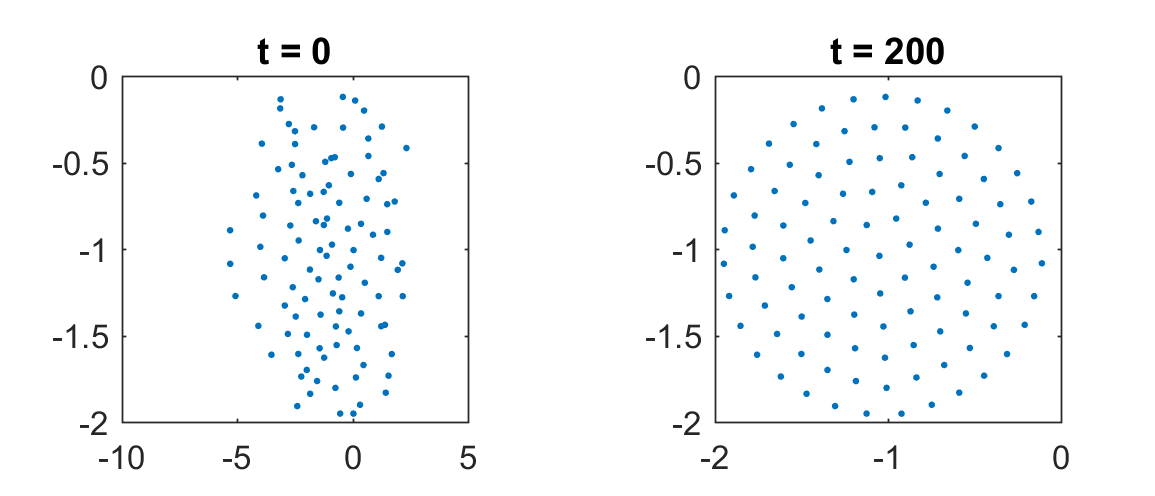
\includegraphics[width=\linewidth]{dim2.png}
\end{figure}


















\section{Set-up on the Sphere}

\subsection{Spherical Coordinates}
Let $\X = x\ei + y\ej + z\ek$ denote the position of a particle in $\R^3$, where $\{\ei,\ej,\ek\}$ is the standard Cartesian basis. Let $R$ be Euclidean norm of $\X$, $\h$ its angle from the z-axis, and $\phi$ its angle from the x-axis. Then we have the following relationship between the coordinate systems
\begin{align*}
x &= R \cos{\phi} \sin{\h}, \\
y &= R \sin{\phi} \sin{\h}, \\
z &= R \cos{\h}.
\end{align*}
Define the standard spherical basis in $\R^3$ as the following:
\begin{align*}
\er &= \frac{\X}{\norm{\X}} = \cos{\phi} \sin{\h} \ei + \sin{\phi} \sin{\h} \ej + \cos{\h} \ek \\
\eh &= \frac{\frac{\p \X}{\p \h}}{\norm{\frac{\p \X}{\p \h}}} = \cos{\phi}\cos{\h} \ei + \sin{\phi}\cos{\h} \ej - \sin{\h}\ek \\
\ep &= \frac{\frac{\p \X}{\p \phi}}{\norm{\frac{\p \X}{\p \phi}} } = -\sin{\phi}\ei + \cos{\phi}\ej
\end{align*}
\subsection{Gradient, Divergence, and the Laplace-Beltrami}

Let $f,g$ be scalar functions on the sphere. And let $F = F_\h \eh + F_{\phi} \ep$ be a vector field on the sphere. Assuming all normal components to the surface of the sphere are zero, gradient, divergence, and Laplace-Beltrami on the sphere are respectively:
\begin{align*}
\nabla f &= \frac{1}{R} \frac{\p f}{\p \h} \eh + \frac{1}{R\sin{\h}} \frac{\p f}{\p \phi} \ep \\
\nabla \cdot F &=\frac{1}{R\sin{\h}} \left(\cos{\h} F_\h + \sin{\h}\frac{\p}{\p\h} F_\h  \right) + \frac{1}{R\sin{\h}} \frac{\p}{\p \phi}F_\phi \\
\Delta f &= \nabla \cdot \nabla f \\
&= \frac{1}{R^2} \left( \cot{\h} \frac{\p f}{\p \h} + \frac{\p^2 f}{\p \h^2} + \frac{1}{\sin^2{\h}} \frac{\p^2 f}{\p \phi^2} \right)
\end{align*}
For an interaction potential that takes two particle positions as arguments, i.e $K(\hi,\phi_i,\hj,\phi_j)$, we define its gradient with respect to $\X_i$ as
\[
\nabla_i K = \frac{1}{R} \frac{\p f}{\p \hi} \ehi + \frac{1}{R\sin{\hi}} \frac{\p f}{\p \phi_i} \epi.
\]
Divergence and Laplacian of $K$ with respect to $\X_i$ are defined similarly.
Finally, convolution centered at $\X_i$ is defined
\[
K * \rho = \int_{0}^{2\pi} \int_{0}^{\pi} K(\hi, \phi_i, \hj, \phi_j) \rho(\hj,\phi_j) R^2 \sin{\hj} d\hj d\phi_j.
\]

\section{Results on the Sphere}
\subsection{Choice of $K$}
Motivated by the \ref{R2Laplacian}, we look for an interaction potential $K$ on the sphere $S$ that satisfies
\[
\Delta_S K = -\delta + C,
\]
where $\Delta_S$ is the Laplace-Beltrami operator on the sphere, and $C$ a constant. As seen in \cite{howard}, for $f$ a test function, we want to solve the convolution equation $\Delta f * K = -f + C \int_S f$. To simplify calculations, assume center of convolution is the north pole: $(\hi = 0, \phi_i = 0)$, then the equation simplifies to: 
\begin{align*}
\int_{0}^{2\pi} \int_{0}^{\pi} \frac{1}{R^2} \left(  \cot{\h} \frac{\p f}{\p \h} + \frac{\p^2 f}{\p\h^2} \right)K(\h) R^2 \sin(\h) d\h d\phi\\
= - f(0,0) + C \int_{0}^{2\pi} \int_{0}^{\pi} f(\h,\phi) R^2 \sin(\h) d\h d\phi.
\end{align*}
We solve for $K$ through integration by parts, moving the partial derivatives on $f$ to $K$ then integrating. We find that it is necessary $C = \frac{1}{4\pi}$, and
\[
\setlength{\fboxsep}{3\fboxsep}\boxed{ K(\tilde{\h}) = -\frac{1}{2\pi} \log{ \sin{ \frac{\tilde{\h}}{2} } } ,}
\]
where $\tilde{\h}$ is the spherical distance between two points. This is, in fact, the generalized Green's function of $\Delta_S$.
\subsection{Analytic Results}
Let $M$ denote total mass in the system. Similar to (\ref{approach}) in the 2-dimensional case, along the characteristic path $X(\alpha,t)$ on the sphere, we have:
\begin{equation}
\label{sphere_approach}
\frac{D}{Dt} \rho =-\rho (\rho - \frac{1}{4\pi}M).
\end{equation}
Again, $\rho_0 = \frac{1}{4\pi}M$ is the global attractor; that is, any initial state will converge to a steady state density of $\rho_0$. Morever, this density must be spread out over the entire surface of the sphere for the system to conserve mass.

\section{Numerical Scheme}
Let $w = \cos{\tilde{\h}}$, where $\tilde{\h}$ is the angle between $\X_i$ and $\X_j$. By law of cosine,
\begin{equation}
w = \cos{\h_i}\cos{\h_j} + \sin{\h_i}\sin{\h_j}\cos{(\phi_i - \phi_j)}
\end{equation}
Then our chosen interaction potential can be written in terms of the spherical coordinates of two points:
\begin{equation}
K(\hi,\phi_i,\hj,\phi_j) = - \frac{1}{2\pi} \log{\left( \sin{ \left( \frac{1}{2} \arccos{w}  \right)   }  \right)}
\end{equation}
Now, the particle-based version of the our equation has the advantage of clear characteristic paths. Let there be $N$ particles in total, each having mass $\frac{1}{N}$. Let $\X_i(t)$ represent the location in $\R^3$ of the $i$-th particle. Then velocity of $\X_i$ can be rewritten from (\ref{velocity}):
\begin{align*}
\frac{d \X_i}{dt} = -\frac{1}{N} \sum_{\substack{j = 1 ... N \\ j \ne i}} \nabla_i K(\X_i,\X_j).
\end{align*}
Expand both sides in spherical basis:
\begin{align*}
\frac{d\X_i}{dt} 
&= \frac{\p \X_i}{\p \h_i}\frac{d\h_i}{dt} + \frac{\p \X_i}{\p \phi_i}\frac{d\phi_i}{dt},\\[0.8ex]
&= R \frac{d \hi}{dt}\ehi + R\sin{\hi} \frac{d \phi_i}{dt} \epi,\\[0.8ex]
\nabla_i K (\X_i,\X_j) &= \frac{1}{R} \frac{\p K}{\p \hi} \ehi + \frac{1}{R\sin{\hi}} \frac{\p K}{\p \phi_i}\epi.
\end{align*}
Compare coefficients of the spherical basis to obtain the ODEs for the spherical coordinate of the $i$-th particle:
\begin{align}
\frac{d \hi}{dt} &= -\frac{1}{N}\sum_{\substack{j=1..N \\ j \neq i}} {\frac{1}{R^2} \frac{\p K}{\p \hi} },\\
\frac{d \phi_i}{dt} &=-\frac{1}{N}\sum_{\substack{j=1..N \\ j \neq i}}{ \frac{1}{R^2\sin^2{\hi}} \frac{\p K}{\p \phi_i}}.
\end{align}
Explicit forward Euler method is used to model the coupled ODEs:
\begin{align*}
\frac{\h_i^{n+1} - \h_i^n}{\Delta t} &= -\frac{1}{N}\sum_{\substack{j=1..N \\ j \neq i}} \frac{1}{R^2} \frac{\p K}{\p \hi} (\h_i^n,\phi_i^n,\h_j^n,\phi_j^n),\\
\frac{\phi_i^{n+1} - \phi_i^n}{\Delta t} &=-\frac{1}{N}\sum_{\substack{j=1..N \\ j \neq i}}  \frac{1}{R^2\sin^2{\hi}} \frac{\p K}{\p \phi_i} (\h_i^n,\phi_i^n,\h_j^n,\phi_j^n).
\end{align*}
\begin{figure}
\centering
\begin{subfigure}{.5\textwidth}
  \centering
  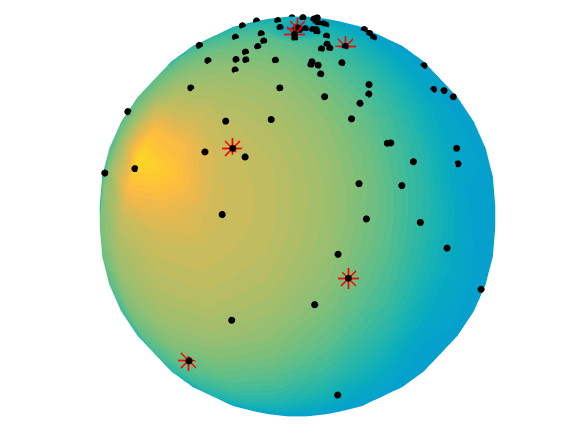
\includegraphics[width=\linewidth]{t_0.png}
  \caption{Initial State}
  \label{fig1}
\end{subfigure}%
\begin{subfigure}{.5\textwidth}
  \centering
  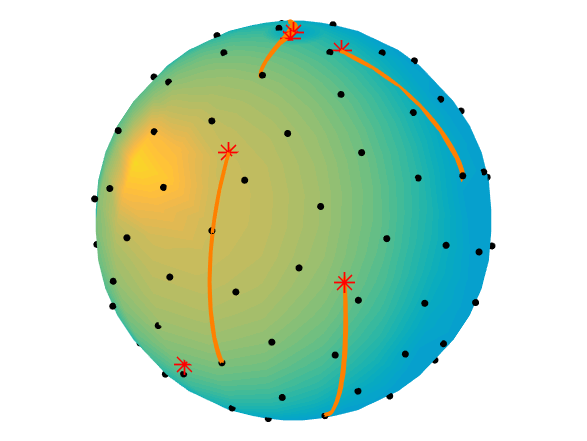
\includegraphics[width=\linewidth]{t_100.png}
  \caption{Steady State, particle paths traced}
  \label{fig2}
\end{subfigure}
\label{fig_main}
\end{figure}

\section{Extensions to Other Surfaces}
\subsection{The same potential on the Hemisphere}
We impose a boundary at $\h=\h_0$ and forbid particles from going beyond it, numerics show that the steady state is:
\begin{itemize}
\item constant density $\rho_0 = \frac{1}{4\pi}M$ in the interior.
\item another constant density depending on $\h_0$ on the boundary, with zero projected velocity. The red arrows denote velocity in the absence of the boundary.
\end{itemize}
\begin{figure}
\centering
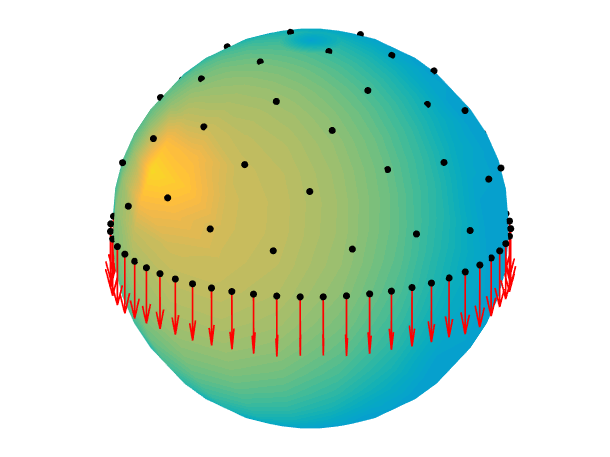
\includegraphics[width=0.5\linewidth]{obstacle.png}
\caption{Equilibrium state with $\h_0=\frac{\pi}{2}$}
\end{figure}
The sphere and the hemisphere share the same local structure, which the gradient, divergence, and Laplace-Beltrami operators depend on. Since (\ref{sphere_approach}) holds true for any surface patch with the same local structure, the interior steady state density is the same.

\subsection{Potentials on the Hyperboloid}
We use the parametrization of the upper sheet of the unit Hyperboloid $\mathbf{H}^2$ from \cite{kimura}:
\begin{align*}
x &= \sinh{\h} \cos{\phi}, \\
y &= \sinh{\h} \sin{\phi}, \\
z &= \cosh{\h}.
\end{align*}
And the following definitions:
\begin{align*}
\Delta f &= \frac{1}{R^2} \left( \coth{\h} \frac{\p f}{\p \h} + \frac{\p^2 f}{\p \h^2} + \frac{1}{\sinh^2{\h}} \frac{\p^2 f}{\p \phi^2} \right),\\
\cosh{\tilde{\h}} &=  \cosh{\h_i}\cosh{\h_j} - \sinh{\h_i}\sinh{\h_j}\cos{(\phi_i - \phi_j)},
\end{align*}
where $\tilde{\h}$ is the hyperbolic distance between two points. Note that hyperbolic distance is not proportional to the arclength visually.

The generalized Green's function to $\Delta$ on the hyperboloid, 
\[
G( \tilde{\h} ) = - \frac{1}{2\pi} \log{ \tanh{\frac{\tilde{\h}}{2}}},
\]
solves $\Delta G = -\delta$. This time, we can add an extra term to get a potential $K$ such that $\Delta K = -\delta + C$. We later see in numerics that $C = \frac{1}{4\pi}$ is again the magic number. $K$ is then explicitly solvable:

\[
\setlength{\fboxsep}{3\fboxsep}\boxed{
K(\tilde{\h}) = -\frac{1}{2\pi} \log{ \tanh{ \frac{\tilde{\h}}{2}}} + \frac{1}{4\pi} \log{ \sinh{ \tilde{\h}}}.
}
\]
This potential leads to a steady state of "constant density in the sense that the hyperbolic distance between particles is even, but not the arc-length distance. Hyperbolic distance can easily be understood by looking at the hyperboloid sheet from an birds-eye view.

The first term of $K$ is repulsive and the second is attractive. In fact, we have convergence to various steady states using the family of attractive terms
\[
A(\tilde{\h})=\frac{1}{4\pi q} \log{ \sinh{ \tilde{\h}^q}}
\]
for $q \in \mathbb{Z}, q \geq 1$.
\begin{figure}
\caption{Birds-eye view of the steady state on the hyperboloid}
\centering
\begin{subfigure}{.5\textwidth}
  \centering
  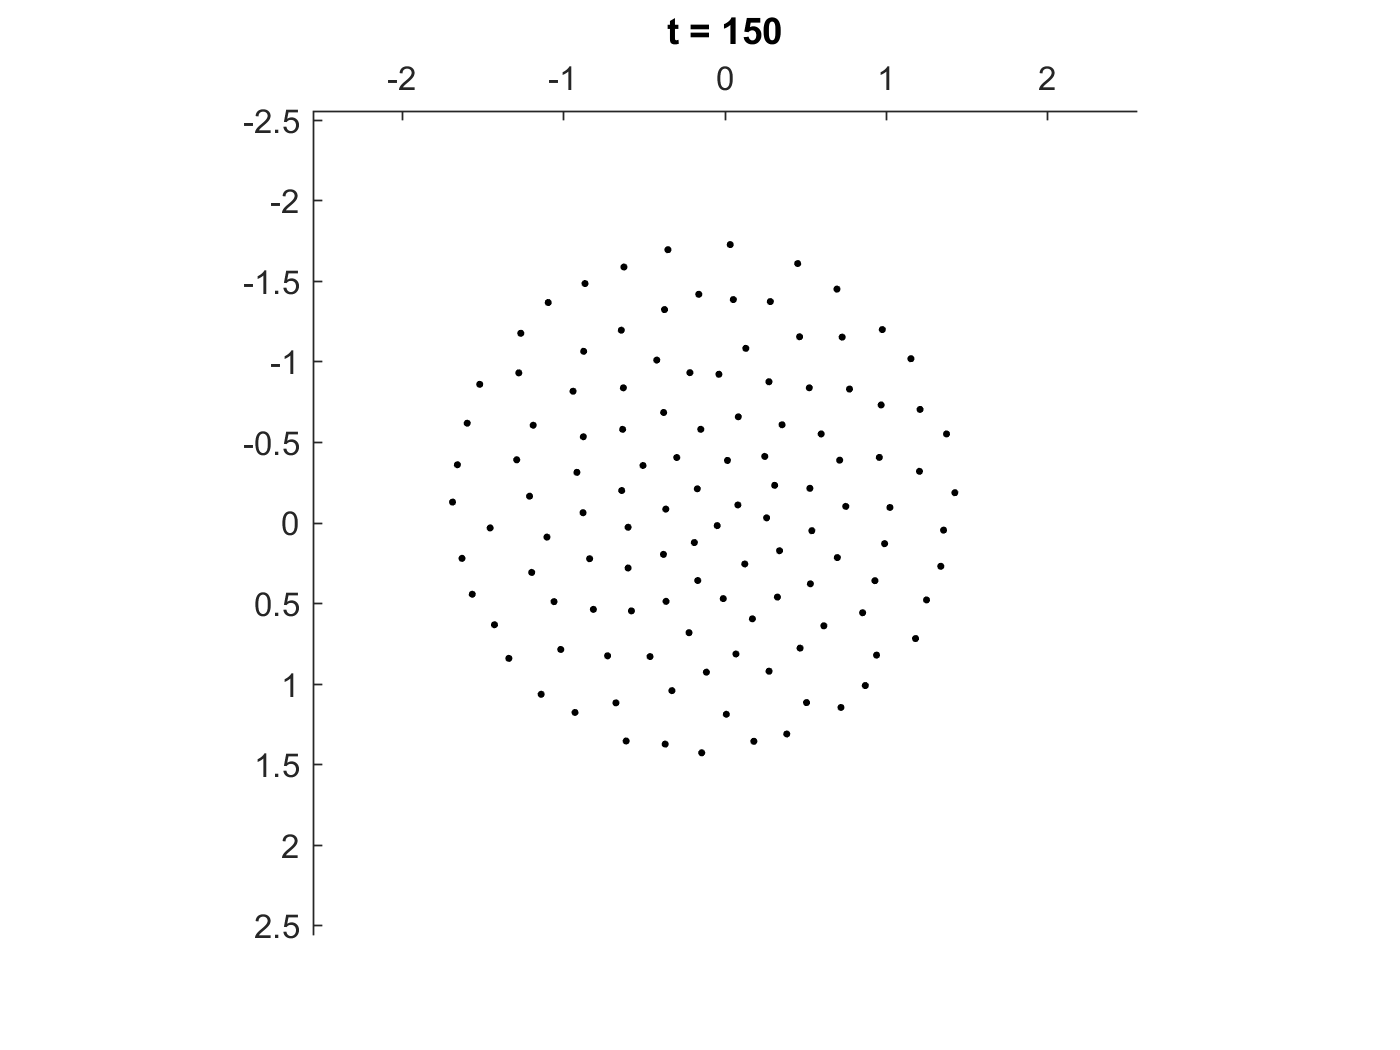
\includegraphics[width=\linewidth]{q1.png}
  \caption{q=1}
\end{subfigure}%
\begin{subfigure}{.5\textwidth}
  \centering
  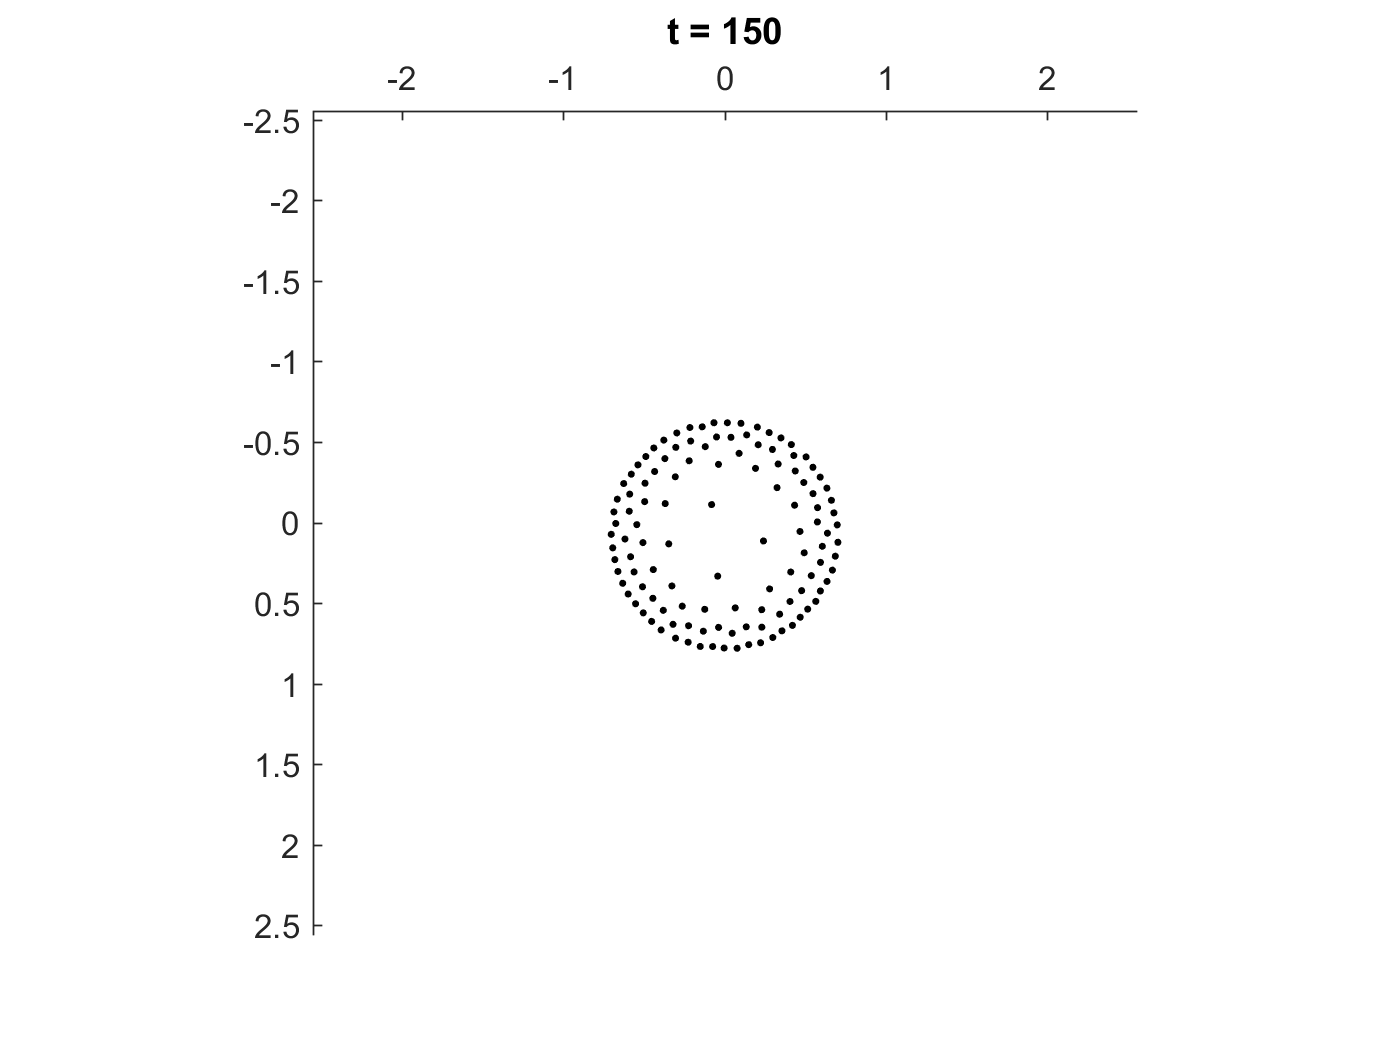
\includegraphics[width=\linewidth]{q8.png}
  \caption{q=8}
\end{subfigure}
\end{figure}

\section{Future Work}
It remains to understand analytically the approach to equilibrium for surfaces other than the sphere.



\begin{thebibliography}{3}
\bibitem{swarm} 
R. C. Fetecau, Y. Huang and T. Kolokolnikov, Swarm dynamics and equilibria for a nonlocal aggregation model , Nonlinearity, Vol. 24, No. 10, 2681-2716 (2011)
 
\bibitem{kimura}
Yoshifumi Kimura, Vortex motion on surfaces with constant curvature, Proc. R. Soc. Lond. A (1999) 455, 245-259

\bibitem{howard}
Cohl, Howard. (2011). Fundamental Solution of Laplace's Equation in Hyperspherical Geometry. Symmetry, Integrability and Geometry: Methods and Applications. 7. . 10.3842/SIGMA.2011.108.

\end{thebibliography}


\end{document}